% !TeX program = pdflatex
% =====================================================================
%  Entregable final — MIA-10 Procesamiento del Lenguaje Natural (UNI)
%  GENERADO AUTOMATICAMENTE por generar_entregable_pln.py
%  NO EDITAR A MANO: las cifras se leen de los resultados del pipeline.
%  Regenerar con:  python generar_entregable_pln.py
% =====================================================================
\documentclass[conference]{IEEEtran}
\IEEEoverridecommandlockouts
\usepackage[utf8]{inputenc}
\usepackage[T1]{fontenc}
\usepackage[spanish,es-tabla]{babel}
\usepackage{graphicx}
\usepackage{booktabs}
\usepackage{amsmath}
\usepackage{url}
\usepackage{cite}

\begin{document}

\title{
\includegraphics[width=2.0cm]{figuras/logo_uni.png}\\[8pt]
Detección automática de eventos adversos hospitalarios\\
en epicrisis mediante Procesamiento de Lenguaje Natural}

\author{\IEEEauthorblockN{Carlos Pérez Pérez}
\IEEEauthorblockA{\textit{Maestría en Inteligencia Artificial}\\
\textit{Universidad Nacional de Ingeniería}\\
Lima, Perú}}

\maketitle

\begin{abstract}
La notificación de eventos adversos en EsSalud depende de un proceso manual y
voluntario con un subregistro estimado cercano al 72\,\%. Este trabajo evalúa
un canal de Procesamiento de Lenguaje Natural que detecta eventos adversos en
resúmenes de alta y los clasifica según la taxonomía del Anexo 02 de la
Directiva GG-ESSALUD-2021, sobre 70,000 epicrisis de MIMIC-IV.
El aporte central no es una métrica sino una auditoría: se identificaron y
corrigieron siete defectos del canal, entre ellos un confusor de época
CIE-9/CIE-10 que producía un caso ejemplar de aprendizaje por atajo, con
AUC 0.973 obtenido al reconocer la plantilla de laboratorio de cada periodo en
lugar del fenómeno clínico. Tras la corrección, el detector alcanza
sensibilidad 0.762 y especificidad 0.770
(AUC 0.843), con un valor predictivo positivo de
0.455 a la prevalencia poblacional
(20.12\%). El contraste con transformers clínicos ajustados
muestra que el factor determinante no es la arquitectura sino la ventana de
contexto: el modelo procesa solo el 9.0\% del documento. La concordancia con un
evaluador independiente alcanza $\kappa$ = 0.644
(IC 95\,\% 0.413--0.817), cuyo valor puntual se sitúa
en la banda sustancial aunque el límite inferior del intervalo no permite
afirmarlo con la muestra disponible.
\end{abstract}

\begin{IEEEkeywords}
procesamiento de lenguaje natural, seguridad del paciente, eventos adversos,
supervisión débil, MIMIC-IV, aprendizaje por atajo
\end{IEEEkeywords}

\section{Introducción}
La seguridad del paciente es un eje crítico de la calidad asistencial desde
que el informe \emph{To Err Is Human} \cite{kohn} situó el daño evitable entre
las principales causas de mortalidad hospitalaria, y desde que el estudio de
Harvard \cite{brennan} estableció la magnitud del fenómeno mediante revisión
manual de historias clínicas. La Organización Mundial de la Salud mantiene la
reducción del daño evitable como objetivo prioritario \cite{who}.

El problema no es solo la ocurrencia sino la \emph{detección}. Classen
\emph{et al.} \cite{classen} demostraron que los métodos voluntarios de
notificación subestiman los eventos adversos hasta en un factor de diez frente
a la revisión sistemática de historias. En EsSalud la notificación es manual,
voluntaria y posterior al hecho: en 2025 se registraron 515\,493 egresos
hospitalarios \cite{cifras} y se notificaron 14\,275 eventos adversos
(2.77\,\%), muy por debajo del 10\,\% estimado internacionalmente. La brecha
---del orden de 37\,000 eventos no notificados en un solo año--- delimita el
problema que este trabajo aborda.

La detección automática sobre texto clínico libre es una línea establecida:
Murff \emph{et al.} \cite{murff} identificaron complicaciones posoperatorias
en historias electrónicas mediante procesamiento de lenguaje natural,
alcanzando sensibilidades muy superiores a la codificación administrativa. Este
trabajo se inscribe en esa línea, con dos particularidades: la taxonomía de
destino es la normativa peruana \cite{directiva02}, \cite{directiva7}, y el
sistema debe operar sobre resúmenes de alta completos.

La propuesta presentada al curso comprometía cuatro objetivos: construir el
corpus mediante supervisión débil con detección de negaciones, comparar un
modelo léxico contra transformers clínicos, mapear los eventos al Anexo 02 y
validar el resultado con un evaluador independiente mediante el coeficiente
$\kappa$ de Cohen \cite{cohen}. Los cuatro se ejecutaron y se reportan aquí,
incluidos los resultados que refutaron las hipótesis iniciales.

\section{Estado del arte}

\subsection{Detección de eventos adversos en texto clínico}
La identificación de eventos adversos ha dependido históricamente de la
revisión manual de historias clínicas, método fiable pero inviable a escala:
el estudio de Harvard \cite{brennan} requirió la lectura de más de 30\,000
historias. La búsqueda de disparadores ---desarrollada por el Institute for
Healthcare Improvement bajo la denominación \emph{Global Trigger Tool}---
acotó el volumen a revisar. Aplicándola, Classen \emph{et al.}
\cite{classen} establecieron que la notificación voluntaria detecta del orden
de una décima parte de los eventos que identifica una revisión sistemática. Murff \emph{et al.} \cite{murff} dieron el paso al procesamiento
automático: aplicando PLN sobre notas clínicas del sistema de veteranos de
EE.\,UU., alcanzaron sensibilidades muy superiores a las de la codificación
administrativa para complicaciones posoperatorias. La conclusión transversal de
esta línea es que el texto libre contiene información que los códigos
administrativos no capturan.

\subsection{Modelos de lenguaje aplicados al dominio clínico}
La arquitectura Transformer \cite{vaswani} y su materialización en BERT
\cite{bert} desplazaron a los métodos léxicos en la mayoría de tareas de PLN.
En el dominio biomédico surgieron variantes preentrenadas sobre corpus
especializados: BioBERT \cite{biobert} sobre PubMed y PMC, Bio\_ClinicalBERT
\cite{clinicalbert} sobre notas clínicas de MIMIC-III, y PubMedBERT
\cite{pubmedbert}, que demostró que el preentrenamiento \emph{desde cero} con
vocabulario del dominio supera a la adaptación de un modelo general. Huang
\emph{et al.} \cite{huang} aplicaron esta familia a la predicción de
reingreso hospitalario. Para el español existe BETO \cite{beto}, que habilita
la transferencia a la lengua de destino sin traducir el corpus.

\subsection{La restricción de la ventana de contexto}
Un límite estructural de esta familia de modelos es la ventana de 512
\emph{tokens}, insuficiente para documentos clínicos completos. Beltagy
\emph{et al.} \cite{longformer} y Zaheer \emph{et al.} \cite{bigbird}
propusieron mecanismos de atención dispersa que reducen el coste cuadrático y
permiten secuencias de hasta 4\,096 \emph{tokens}. Li \emph{et al.}
\cite{cliniclong} llevaron esa idea al dominio clínico y mostraron que
Clinical-Longformer supera consistentemente a ClinicalBERT en clasificación
documental. Esta línea es directamente pertinente para el presente trabajo,
como se cuantifica en la Sección~\ref{sec:ventana}.

\subsection{Supervisión débil y etiquetado programático}
La anotación manual de corpus clínicos extensos es prohibitiva. El paradigma de
\emph{supervisión débil} formalizado en Snorkel \cite{snorkel} sustituye la
anotación por funciones de etiquetado que codifican reglas heurísticas,
aceptando ruido a cambio de escala. En texto clínico, el tratamiento de la
negación es imprescindible: el algoritmo NegEx \cite{negex} sigue siendo la
referencia para distinguir la mención de un hallazgo de su afirmación.

\subsection{Validez de las mediciones y aprendizaje por atajo}
Un cuerpo creciente de literatura advierte que las métricas altas pueden
sostenerse en correlaciones espurias. Geirhos \emph{et al.} \cite{geirhos}
sistematizaron el fenómeno como \emph{shortcut learning}, y Zech \emph{et
al.} \cite{zech} documentaron el caso clínico canónico: un detector de
neumonía en radiografías que había aprendido a identificar el hospital de
procedencia. Esta literatura motiva la auditoría que constituye el aporte
central de este trabajo.

\subsection{Medición de la fiabilidad entre observadores}
Cuando la referencia es un juicio humano, la concordancia se mide con el
coeficiente $\kappa$ de Cohen \cite{cohen}, interpretado según la escala de
Landis y Koch \cite{landis}. Feinstein y Cicchetti \cite{feinstein}
demostraron que con prevalencias extremas el coeficiente se deprime pese a un
acuerdo observado alto, y Byrt \emph{et al.} \cite{byrt} propusieron el
PABAK para corregir ese efecto. Sim y Wright \cite{sim} sistematizaron los
requisitos de tamaño muestral y de reporte del intervalo de confianza, que en
este trabajo se estima por \emph{bootstrap} \cite{efron}.

\subsection{Síntesis y brechas de investigación}
El estado del arte evidencia tres brechas que este trabajo aborda. Primera:
los estudios de detección automática de eventos adversos rara vez auditan la
validez de su propia etiqueta, pese a que se construye por reglas sobre
codificación administrativa. Segunda: la comparación entre modelos léxicos y
transformers clínicos suele reportarse sin controlar la asimetría en la
cantidad de texto que cada arquitectura procesa, lo que confunde el efecto del
modelo con el de la ventana de contexto. Tercera: las taxonomías empleadas son
mayoritariamente anglosajonas, mientras que la aplicación institucional exige
la taxonomía normativa local \cite{directiva02}, \cite{directiva7}, sobre la
que casi no existen corpus etiquetados.

\section{Problemática}
La notificación de eventos adversos en EsSalud opera de forma reactiva: depende
de que un profesional decida reportar, tras el hecho y de manera voluntaria. La
consecuencia medible es un subregistro cercano al 72\,\%, equivalente a unos
37\,000 eventos no reportados en un solo año. Esos eventos no solo no se
gestionan: son invisibles para la planificación de la calidad, lo que impide
priorizar intervenciones, dimensionar el riesgo y anticipar la exposición
sancionatoria.

El obstáculo no es la ausencia de información, sino su formato. La descripción
de lo ocurrido existe en las epicrisis, redactada en texto libre, pero no en
una forma explotable de manera automática. De ahí la pregunta de investigación:

\begin{quote}
\emph{¿Es posible detectar automáticamente, a partir del texto libre de los
resúmenes de alta, los eventos adversos ocurridos durante la hospitalización, y
clasificarlos según la taxonomía normativa vigente, con una fiabilidad
comparable a la del juicio experto?}
\end{quote}

Responderla exige resolver tres problemas encadenados: construir una etiqueta
de referencia sin anotación manual exhaustiva, verificar que el modelo aprende
el fenómeno clínico y no un artefacto documental, y demostrar que el criterio
aplicado es reproducible por un evaluador independiente.

\section{Corpus y método}
Se emplea MIMIC-IV-Note v2.2 \cite{mimic4}, alojada en PhysioNet
\cite{physionet}, con 331\,793 resúmenes de alta en inglés del Beth Israel
Deaconess Medical Center (2008--2019). El corpus de modelado quedó en
70,000 epicrisis (37,692 positivas), techo impuesto
por la memoria disponible al vectorizar $n$-gramas de carácter. La prevalencia
poblacional del evento codificado es 20.12\%:
109,775 hospitalizaciones \emph{con} evento sobre un
universo de 545,601
hospitalizaciones registradas en el módulo hospitalario.

El etiquetado sigue el paradigma de \textbf{supervisión débil}
\cite{snorkel}: reglas sobre códigos diagnósticos y patrones textuales generan
etiquetas de forma programática, sin anotación manual exhaustiva. Las
negaciones se tratan con el algoritmo NegEx \cite{negex}, imprescindible en
texto clínico donde la mención de una complicación suele aparecer negada
(\emph{no evidence of infection}).

La partición se realiza \textbf{por paciente} mediante \texttt{GroupShuffleSplit}
sobre \texttt{subject\_id}, con verificación explícita de que ningún paciente
aparece simultáneamente en entrenamiento y prueba. La vectorización TF-IDF se
ajusta únicamente sobre el conjunto de entrenamiento. La implementación emplea
scikit-learn \cite{sklearn} y la biblioteca \emph{Transformers} \cite{hf}.

\section{Validez del etiquetado y control de sesgos}
El etiquetado por supervisión débil \cite{snorkel} traslada la calidad del
corpus a la calidad de las reglas, de modo que su validez debe verificarse de
forma explícita y no presuponerse. Se aplicó un protocolo sistemático de
control que identificó siete \emph{modos de fallo}, cada uno con su efecto
cuantificado sobre el corpus resultante (Tabla~\ref{tab:defectos}). El
procedimiento es reproducible y los modos de fallo son generalizables a
cualquier canal de PLN clínico construido sobre reglas.

\begin{table}[htbp]
\caption{Modos de fallo del etiquetado por reglas y efecto medido}
\label{tab:defectos}
\centering
\footnotesize
\begin{tabular}{@{}p{0.42\columnwidth}p{0.48\columnwidth}@{}}
\toprule
\textbf{Defecto} & \textbf{Efecto medido} \\
\midrule
Muestreo no declarado: se examinaba el 9\,\% del corpus & 301\,793 epicrisis sin revisar \\
\texttt{re.DOTALL}: el comodín cruzaba la epicrisis completa & $-63.7$\,\% de detecciones \\
Códigos CIE-10 con punto frente a MIMIC sin punto & Corpus positivo $\times$267 \\
Ausencia de clase negativa & Abstención 6/6 ante texto trivial \\
\textbf{Confusor de época CIE-9/CIE-10} & Ver Secc.~\ref{sec:atajo} \\
43 de 223 códigos eran reglas muertas (OMS $\neq$ CM) & Medicación $\times$68 \\
Percentiles degenerados con $n$ pequeño & Inversión de prioridad \\
\bottomrule
\end{tabular}
\end{table}

La evidencia decisiva del segundo defecto: los patrones que contenían
\texttt{.*} cayeron $-84.1$\,\% al acotar su alcance (42\,330 a 6\,735),
mientras que los patrones sin comodín quedaron \emph{idénticos}
(13\,189 a 13\,189). La pérdida provenía del alcance del comodín y no de la
especificidad de los patrones.

\subsection{El confusor de época: aprendizaje por atajo}
\label{sec:atajo}
El mapeo inicial contenía únicamente códigos CIE-10. Dado que MIMIC-IV abarca
2008--2019, toda hospitalización de la era CIE-9 resultaba negativa \emph{por
construcción}: los negativos eran 78.97\,\% de la era CIE-9 y los positivos
100\,\% de la era CIE-10.

El clasificador no aprendió a reconocer eventos adversos sino la plantilla de
laboratorio de cada época. El rasgo de mayor peso resultó ser
\texttt{palabra\_\_rdwsd}, un artefacto de cabecera sin contenido clínico. Es un
caso de \emph{shortcut learning} \cite{geirhos}: el modelo explota una
correlación espuria disponible en los datos en lugar del fenómeno que se
pretende medir, y obtiene métricas excelentes que no generalizan. El paralelo
más conocido en el ámbito clínico es el de Zech \emph{et al.} \cite{zech},
cuyo detector de neumonía en radiografías aprendió a reconocer el hospital de
procedencia a partir de marcas en la imagen (Tabla~\ref{tab:epoca}).

\begin{table}[htbp]
\caption{Efecto del confusor de época sobre las métricas}
\label{tab:epoca}
\centering
\footnotesize
\begin{tabular}{@{}lccc@{}}
\toprule
\textbf{Versión} & \textbf{Espec.} & \textbf{AUC} & \textbf{VPP} \\
\midrule
Inicial (inválida, no se cita) & 0.917 & 0.973 & 0.433 \\
Reevaluada con emparejamiento & 0.694 & 0.904 & 0.171 \\
\textbf{Final, siete defectos corregidos} & \textbf{0.770} & \textbf{0.843} & \textbf{0.455} \\
\bottomrule
\end{tabular}
\end{table}

La corrección consistió en extender el mapeo a CIE-9 (996--999\,$\approx$\,T80--T88,
E870--E879\,$\approx$\,Y60--Y69, E930--E949\,$\approx$\,Y40--Y59,
707.0x\,$\approx$\,L89) y en forzar el emparejamiento \textbf{a nivel de nota} y
no de hospitalización, dado que la cobertura de epicrisis difiere entre eras.
El emparejamiento resultante es exacto:
28.92\% frente a
28.92\%. Tras la corrección los
rasgos de mayor peso pasaron a ser inequívocamente clínicos (\emph{fall}, \emph{induced}, \emph{ileus}, \emph{revision}, \emph{in stent}, \emph{pressure ulcer}, \emph{restenosis}, \emph{reaction}) y el
artefacto documental desapareció del modelo.

\section{Evaluación de los modelos}
La evaluación se diferencia según la etapa del canal y el objetivo de gestión,
con métricas elegidas de forma explícita y no por convención.

\subsection{Métricas de la etapa de detección y su justificación}
La exactitud global es engañosa en esta tarea: con una prevalencia poblacional
del 20.12\%, un clasificador que negara todo evento
alcanzaría más del 79\,\% de aciertos sin detectar un solo caso. Se reportan por
tanto métricas sensibles al desbalance:

\begin{itemize}
\item \textbf{Sensibilidad}. Es la métrica prioritaria desde la perspectiva de
gestión: omitir un evento adverso (falso negativo) tiene un coste asistencial y
sancionatorio muy superior al de revisar un caso que no lo era.
\item \textbf{Especificidad}. Controla el volumen de revisión que el sistema
impone al servicio de calidad; una especificidad baja lo haría inoperante por
saturación.
\item \textbf{AUC}. Resume la capacidad discriminativa con independencia del
umbral, lo que permite comparar modelos sin fijar un punto de operación.
\item \textbf{Valor predictivo positivo a prevalencia real}. El conjunto de
prueba está balanceado por construcción, de modo que su VPP bruto sobreestima
el operativo. Se reajusta a la prevalencia poblacional mediante el teorema de
Bayes, porque es la cifra que determina cuántas revisiones improductivas
generaría el sistema en producción.
\end{itemize}

Para la clasificación de la naturaleza se prioriza el \textbf{F1-macro} sobre
el F1-micro: al promediar sin ponderar por frecuencia, penaliza el abandono de
las clases minoritarias, que en seguridad del paciente son precisamente las de
mayor gravedad.

\subsection{Protocolo de evaluación y control de fuga}
Tres decisiones de protocolo condicionan la validez de las cifras:

\begin{enumerate}
\item \textbf{Partición por paciente.} Un mismo paciente puede aportar varias
notas con vocabulario e historia compartidos. La partición se realiza con
\texttt{GroupShuffleSplit} agrupando por \texttt{subject\_id}, con una
aserción explícita que verifica la ausencia de solape. Particionar por nota
inflaría las métricas.
\item \textbf{Ajuste del vectorizador solo en entrenamiento.} El vocabulario y
los pesos TF-IDF se estiman exclusivamente sobre el conjunto de entrenamiento.
\item \textbf{Intervalos por \emph{bootstrap} agrupado.} Los intervalos de
confianza se calculan remuestreando \emph{pacientes} y no notas
\cite{efron}: con 1.13 veces de
ensanchamiento respecto del remuestreo ingenuo, el efecto es moderado pero
real, y omitirlo produciría intervalos artificialmente estrechos.
\end{enumerate}

\subsection{Evaluación de la concordancia con criterio humano}
Dado que la etiqueta de MIMIC es un estándar de plata, la evaluación se
completa con la concordancia frente a un evaluador independiente, medida con el
coeficiente $\kappa$ de Cohen \cite{cohen} e interpretada según Landis y Koch
\cite{landis}. Se reporta acompañado del acuerdo observado, del PABAK
\cite{byrt} y de los índices de prevalencia y sesgo, siguiendo la
recomendación de Sim y Wright \cite{sim} para evitar la interpretación errónea
del coeficiente en escenarios desbalanceados \cite{feinstein}.

\section{Resultados}
\subsection{Detección binaria}
\label{sec:deteccion}
Vectorización TF-IDF (palabra y carácter) con LinearSVC balanceado. Los
intervalos se calculan por \textbf{bootstrap agrupado por paciente}: remuestrear
notas sueltas viola la independencia, porque un mismo paciente aporta varias
notas al conjunto de prueba (Tabla~\ref{tab:deteccion}).

\begin{table}[htbp]
\caption{Etapa de detección. IC por bootstrap agrupado por paciente}
\label{tab:deteccion}
\centering
\footnotesize
\begin{tabular}{@{}lcc@{}}
\toprule
\textbf{Métrica} & \textbf{Valor} & \textbf{IC 95\,\%} \\
\midrule
Sensibilidad & 0.762 & [0.751--0.773] \\
Especificidad & 0.770 & [0.759--0.781] \\
AUC & 0.843 & [0.836--0.849] \\
VPP (prevalencia real) & \textbf{0.455} & --- \\
\bottomrule
\end{tabular}
\end{table}

El conjunto de prueba está balanceado, por lo que su VPP bruto (0.793)
sobreestima el operativo. Se reporta el VPP reajustado a la prevalencia
poblacional, que es la cifra con la que trabajaría un servicio de calidad.
Ante seis textos triviales o sin contenido clínico el detector se abstuvo en
6 de 6 casos. La Figura~
ef{fig:roc} muestra la curva ROC con el
punto de operación empleado y la Figura~
ef{fig:confusion} el reparto de
aciertos y errores.

\begin{figure}[htbp]
\centering
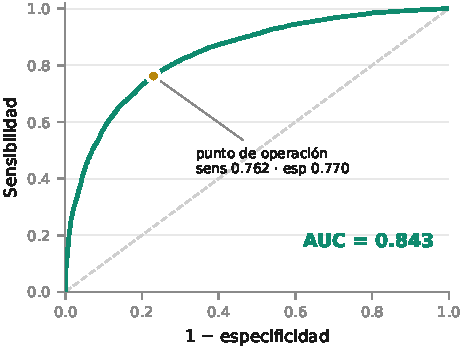
\includegraphics[width=\columnwidth]{figuras/fig1_roc.pdf}
\caption{Curva ROC del detector sobre el conjunto de prueba. El punto marcado
corresponde al umbral por defecto empleado en operación.}
\label{fig:roc}
\end{figure}

\begin{figure}[htbp]
\centering
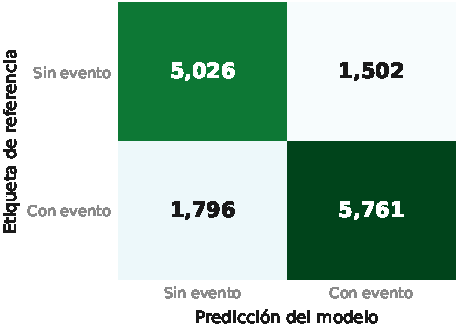
\includegraphics[width=0.86\columnwidth]{figuras/fig2_confusion.pdf}
\caption{Matriz de confusión de la etapa de detección. Los falsos negativos
(esquina inferior izquierda) son el error crítico desde la perspectiva de
gestión de la seguridad del paciente.}
\label{fig:confusion}
\end{figure}

\subsection{Clasificación de la naturaleza y evaluación en cascada}
Evaluar la clasificación sobre positivos \emph{de referencia} supone un
detector perfecto y sobreestima el rendimiento real. Se reporta por tanto la
cascada completa texto\,$\rightarrow$\,detección\,$\rightarrow$\,naturaleza
(Tabla~\ref{tab:cascada}).

\begin{table}[htbp]
\caption{Clasificación aislada frente a cascada extremo a extremo}
\label{tab:cascada}
\centering
\footnotesize
\begin{tabular}{@{}lcc@{}}
\toprule
\textbf{Evaluación} & \textbf{F1-micro} & \textbf{F1-macro} \\
\midrule
Aislada (positivos de referencia) & 0.752 & 0.513 \\
\textbf{Cascada extremo a extremo} & \textbf{0.493} & \textbf{0.363} \\
\bottomrule
\end{tabular}
\end{table}

La caída es de 34.5\,\% en F1-micro. Se calculó sobre las
6,655 notas (47.2\% del conjunto de prueba)
cuyos pacientes no fueron vistos por \emph{ninguna} de las dos etapas: como cada
etapa se particionó por separado, evaluar la cascada sobre todo el conjunto
habría constituido fuga de información.

\subsection{Comparación con transformers clínicos}
La comparación de mayo concluyó que el modelo léxico superaba al transformer
clínico. Al completarla en condiciones controladas, esa conclusión
\textbf{no se sostiene}: procedía de dos asimetrías no declaradas que
favorecían al modelo léxico. Documentarlas importa más que el ranking mismo,
porque son errores frecuentes al comparar familias de modelos.

\emph{Primera asimetría: la ventana de contexto.} La arquitectura BERT
\cite{bert}, \cite{vaswani} limita la entrada a un número fijo de
\emph{tokens}. Con la ventana empleada, el transformer accede al
9.0\% del documento ---la epicrisis mediana tiene
3,148 \emph{tokens}--- mientras que TF-IDF lo procesa
íntegro.

\emph{Segunda asimetría: la ponderación de clases.} El modelo léxico se
entrenó con pesos inversamente proporcionales a la frecuencia; el ajuste fino
inicial de los transformers empleó entropía cruzada sin ponderar. Dado que el
F1-macro penaliza el abandono de las clases minoritarias, esa diferencia de
preprocesamiento castiga al transformer en la métrica principal.

Corregidas ambas ---añadiendo variantes léxicas sin balanceo y reentrenando
Bio\_ClinicalBERT con pesos de clase--- se obtiene el ranking de la
Tabla~\ref{tab:modelos}, con todos los modelos sobre la misma partición.

\begin{table*}[htbp]
\caption{Ranking de desempeño de los modelos evaluados sobre la misma
partición estratificada (semilla 42), ordenado por F1-macro}
\label{tab:modelos}
\centering
\footnotesize
\begin{tabular}{@{}clccc@{}}
\toprule
\textbf{\#} & \textbf{Modelo} & \textbf{Exactitud} & \textbf{F1-macro} & \textbf{$\kappa$} \\
\midrule
1 & \textbf{TF-IDF + LinearSVC (texto completo)} & 0.715 & 0.459 & 0.544 \\
2 & \textrm{TF-IDF + LinearSVC sin balanceo (texto completo)} & 0.711 & 0.391 & 0.513 \\
3 & \textrm{Bio\_ClinicalBERT (fine-tuning, ponderado)} & 0.543 & 0.354 & 0.325 \\
4 & \textrm{TF-IDF + LinearSVC (truncado a 1150 car.)} & 0.575 & 0.330 & 0.315 \\
5 & \textrm{TF-IDF + LinearSVC sin balanceo (truncado a 1150 car.)} & 0.589 & 0.275 & 0.295 \\
6 & \textrm{Bio\_ClinicalBERT (fine-tuning)} & 0.607 & 0.249 & 0.344 \\
7 & \textrm{BioBERT (fine-tuning)} & 0.597 & 0.210 & 0.318 \\
\bottomrule
\end{tabular}
\end{table*}

La tabla incorpora las variantes léxicas \emph{con} y \emph{sin} ponderación
de clases. La distinción no es cosmética: el ajuste fino de los transformers
emplea entropía cruzada sin ponderar, de modo que compararlos contra un modelo
léxico balanceado atribuiría al modelo una ventaja que procede del
preprocesamiento. Las filas «sin balanceo» son las emparejadas.

\subsubsection{A igualdad de condiciones, el transformer no queda por debajo}
Restringiendo la comparación a los modelos que ven la misma cantidad de texto
y emplean ponderación de clases, Bio\_ClinicalBERT ajustado alcanza F1-macro
0.354 frente a 0.330 del modelo léxico truncado. La
ponderación resulta decisiva para el transformer: sin ella su F1-macro cae a
0.249, una diferencia del 42\% atribuible únicamente
al tratamiento del desbalance. La conclusión de que «el modelo simple gana»
era, en esa parte, un artefacto del protocolo.

\subsubsection{La ventana de contexto sí explica la diferencia real}
\label{sec:ventana}
La arquitectura BERT \cite{bert}, \cite{vaswani} limita la entrada a un
número fijo de \emph{tokens} ---512 en su configuración estándar---. Por
restricciones de memoria de la GPU disponible, este experimento se ejecutó con
una ventana de 256 \emph{tokens}. Dado que las
epicrisis del corpus tienen una mediana de 3,148
\emph{tokens}, el transformer accede únicamente al
9.0\% del documento, mientras que TF-IDF lo procesa
íntegro. Atribuir la diferencia a la arquitectura sin controlar esa asimetría
sería un error de interpretación. Con la ventana estándar de 512 la cobertura
seguiría siendo minoritaria (en torno al 16\,\%), de modo que la conclusión no
depende de esta restricción.

Para separar ambos efectos se entrenó el modelo léxico sobre el texto
\textbf{truncado a la misma ventana}. Su F1-macro cae de
0.391 a 0.275, una pérdida de
0.116 puntos (29.7\% en términos relativos), \emph{con la misma
arquitectura y los mismos datos}. Es decir, una fracción sustancial de la
desventaja observada en los transformers no proviene del modelo sino de cuánto
texto alcanza a leer.

\begin{figure}[htbp]
\centering
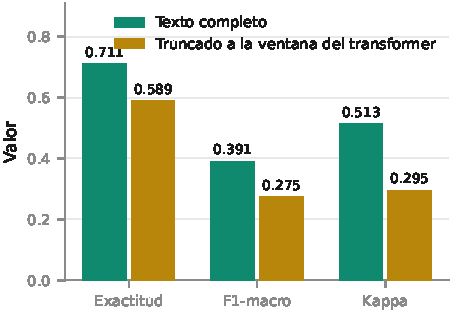
\includegraphics[width=\columnwidth]{figuras/fig3_ventana.pdf}
\caption{Efecto aislado de la ventana de contexto. Mismo algoritmo y mismos
datos; lo único que cambia es cuánto texto procesa el modelo.}
\label{fig:ventana}
\end{figure}

El efecto se representa en la Figura~
ef{fig:ventana}. Concuerda con la
literatura sobre documentos clínicos largos:
Beltagy \emph{et al.} \cite{longformer} y Zaheer \emph{et al.}
\cite{bigbird} propusieron mecanismos de atención dispersa precisamente para
superar ese límite, y Li \emph{et al.} \cite{cliniclong} mostraron que
extender la ventana de 512 a 4\,096 \emph{tokens} sobre corpus clínicos
supera de forma consistente a ClinicalBERT en clasificación documental. La
implicación práctica para este trabajo es directa: la vía de mejora no pasa por
un preentrenamiento clínico más específico \cite{pubmedbert}, \cite{huang},
sino por una arquitectura capaz de abarcar el documento completo.

\subsubsection{Vigencia de las cifras previas}
Las mediciones de mayo (exactitud 0.731, F1-macro 0.515, $\kappa$ 0.581 para
TF-IDF con LinearSVC) son anteriores a la corrección del sexto defecto, que
alteró el reparto de clases. Se conservan por transparencia, pero los valores
de la Tabla~\ref{tab:modelos}, obtenidos todos sobre la misma partición y en
la misma ejecución, son los comparables entre sí.

\subsection{Contraste con trabajos previos}
La comparación numérica directa con la literatura \textbf{no es
metodológicamente admisible} en este caso, y conviene argumentar por qué en
lugar de forzar una tabla de cifras que induzca a error.

Los trabajos de referencia validan contra \emph{revisión manual de historias
clínicas}, que es un estándar de oro; las métricas de este trabajo se calculan
contra \emph{códigos CIE}, que constituyen un estándar de plata. Una
sensibilidad medida frente a un revisor humano y otra medida frente a una
regla de codificación no son la misma magnitud, aunque compartan nombre.
Difieren además el corpus, el idioma, el sistema sanitario, la taxonomía de
destino y el conjunto de complicaciones consideradas.

Lo que sí puede establecerse es la posición cualitativa del enfoque:

\begin{itemize}
\item Murff \emph{et al.} \cite{murff} reportan que el procesamiento de
lenguaje natural sobre notas clínicas alcanza una \textbf{sensibilidad
superior y una especificidad inferior} a la de los indicadores de seguridad
del paciente derivados de la codificación al alta. El presente trabajo comparte
ese régimen de funcionamiento: sensibilidad y especificidad quedan
equilibradas (0.762 y 0.770) y muy por
encima de lo que la codificación administrativa alcanza por sí sola, aunque el
punto de operación no se optimizó ---se mantuvo el umbral por defecto del
clasificador---.
\item Classen \emph{et al.} \cite{classen} establecieron que los métodos
basados en notificación voluntaria detectan del orden de \textbf{una décima
parte} de los eventos que identifica una revisión sistemática. Ese es el
margen de subregistro que un sistema automático aspira a cubrir, y el que
justifica el enfoque.
\item El \emph{Global Trigger Tool} alcanza una detección más completa, pero
exige revisión humana de cada caso disparado: no compite en el mismo régimen
de coste, sino que define el techo al que un sistema automático se aproxima.
\end{itemize}

La vía para hacer comparable este trabajo con esa literatura es sustituir el
estándar de plata por juicio experto, que es exactamente el objeto de la
validación reportada en la sección siguiente.

\section{Validación con evaluador independiente}
La propuesta comprometía un segundo evaluador independiente sobre una
submuestra, midiendo la concordancia con el coeficiente $\kappa$ de Cohen. Se
ejecutó sobre una muestra ciega estratificada, con una interfaz que oculta el
veredicto del sistema, el código diagnóstico de origen y el estrato, y con
registro automático del tiempo dedicado a cada caso.

\textbf{Protocolo de lectura.} Ambos evaluadores dispusieron de la
\emph{epicrisis completa}. La interfaz presenta en primer plano las secciones
de evolución hospitalaria y diagnósticos al alta ---donde la norma documental
de MIMIC sitúa las complicaciones--- y mantiene el texto íntegro accesible de
forma inmediata. La presentación sigue una regla estructural fija, idéntica
para todos los casos e independiente del veredicto del sistema, de modo que no
introduce sesgo hacia la predicción del modelo. El manual de anotación exige
además \emph{cita literal} del fragmento que sustenta todo veredicto positivo,
lo que obliga a recurrir al texto completo cuando el resumen inicial no basta.
Todas las anotaciones se realizaron aplicando el manual reconciliado con la
directiva institucional; una fase piloto previa, anterior a la existencia de
dicho manual, se trató por separado y no se integró en el cálculo de
concordancia.

Sobre 78 casos doble-anotados el acuerdo observado es
0.872 y el coeficiente $\kappa$ = 0.644
(IC 95\,\% 0.413--0.817), situado en la banda
\emph{sustancial} de Landis y Koch. El límite inferior del intervalo queda por
debajo del umbral de 0.61 por efecto del tamaño muestral, por lo que la
afirmación se enuncia con esa reserva. El índice de prevalencia es
0.538: con clases tan desbalanceadas el coeficiente se
deprime (paradoja de Feinstein--Cicchetti), razón por la cual se reporta junto
al PABAK (0.744) y al acuerdo observado. La prueba de McNemar no
detecta sesgo sistemático entre evaluadores ($p$ = 0.34).

\subsection{Concordancia en la naturaleza del evento}
Sobre los casos en que ambos evaluadores coincidieron en la existencia del
evento ($n$ = 55), la concordancia en su \emph{naturaleza}
resulta $\kappa$ = 0.281
(IC 95\,\% 0.029--0.654),
con un acuerdo exacto de 0.855.

Este coeficiente \textbf{no es interpretable} en la presente muestra, y se
reporta precisamente para dejar constancia de ello. La discrepancia entre un
acuerdo observado alto y un $\kappa$ bajo obedece a la concentración extrema de
la variable: la muestra de validación está restringida a eventos de infección
por construcción, de modo que casi todos los casos comparten una misma
naturaleza y el acuerdo esperado por azar se aproxima a la unidad. Es la
paradoja descrita por Feinstein y Cicchetti \cite{feinstein} llevada al
límite. Estimar la concordancia en naturaleza exigiría una muestra
estratificada sobre las doce categorías, no sobre el veredicto binario.

\section{Clasificación del corpus ERSP en español con etiqueta de oro}
\label{sec:ersp}

\subsection{Motivación: estándar de plata frente a estándar de oro}
Las etiquetas del corpus MIMIC se derivan de codificación administrativa CIE:
el modelo aprende a predecir códigos, no juicios clínicos, y constituyen por
tanto un \emph{estándar de plata}. Toda métrica de las secciones anteriores
hereda esa limitación.

Para contrastar el enfoque contra criterio humano se incorporó un segundo
corpus, en español y sobre la taxonomía peruana: 8,799
ocurrencias notificadas al sistema institucional de reporte de eventos
adversos, en las que profesionales expertos ---con formación en gestión de la
calidad, seguridad del paciente y auditoría médica--- leyeron la descripción
textual y codificaron, una a una, el tipo de evento, la naturaleza según el
Anexo 02 y la severidad según el Anexo 03. Es un \emph{estándar de oro}: juicio
humano especializado, en el idioma y bajo la norma de destino del sistema.

\subsection{Preprocesamiento}
El texto libre exigió tres correcciones antes de modelar:
\begin{itemize}
\item \textbf{Anonimización.} Las columnas no contenían identificadores, pero la
narrativa sí: se retiraron 124 secuencias numéricas
compatibles con documentos de identidad, además de nombres propios asociados,
iniciales e instituciones nombradas, sustituidos por marcadores. Los casos que
no admitían regla automática sin riesgo de borrar vocabulario clínico se
marcaron para revisión humana en lugar de silenciarse.
\item \textbf{Deduplicación.} 2,463
registros resultaron duplicados o demasiado breves; el corpus quedó en
6,336 textos únicos. Sin este paso el mismo texto aparecía en
entrenamiento y prueba, inflando artificialmente las métricas.
\item \textbf{Normalización de etiquetas} y descarte de las clases con menos de
50 ejemplos, declaradas no modelables.
\end{itemize}

Se aplicó partición estratificada 80/20 con verificación explícita de que
ningún texto aparece en ambos conjuntos, y vectorización TF-IDF de unigramas y
bigramas con supresión de acentos.

\subsection{Tareas y resultados}
El corpus permite tres tareas que el corpus MIMIC no puede sostener
(Tabla~\ref{tab:oe5}).

\begin{table}[htbp]
\caption{Tareas de clasificación sobre el corpus ERSP (etiqueta de oro)}
\label{tab:oe5}
\centering
\footnotesize
\begin{tabular}{@{}lccccc@{}}
\toprule
\textbf{Tarea} & \textbf{$n$} & \textbf{Cl.} & \textbf{Modelo} & \textbf{F1-mac.} & \textbf{F1-mic.} \\
\midrule
Binaria & 6,334 & 2 & LogReg & \textbf{0.860} & 0.864 \\
Naturaleza & 6,276 & 9 & LinearSVC & \textbf{0.767} & 0.845 \\
Severidad & 6,279 & 4 & LogReg & \textbf{0.606} & 0.725 \\
\bottomrule
\end{tabular}
\end{table}

\textbf{Tarea 1: evento adverso frente a incidente.} Es la distinción central
de la norma ---si hubo o no daño al paciente--- y \emph{no puede medirse sobre
MIMIC}, porque un resumen de alta no documenta los cuasi-incidentes. El
corpus ERSP sí los contiene, con clases casi balanceadas, y la tarea alcanza
F1-macro 0.860. Es la primera evidencia del trabajo de que el criterio nuclear
del codebook es aprendible automáticamente.

\textbf{Tarea 2: naturaleza del evento.} Es la tarea homóloga a la
Sección~\ref{sec:atajo} pero con etiqueta humana. Nueve de las doce
naturalezas superan el umbral de 50 ejemplos, cubriendo el 99.1\,\% de los
registros. El desglose por clase (Tabla~\ref{tab:oe5clases}) muestra un
resultado relevante para la tesis: \emph{Gestión de la organización}, que en
MIMIC era inviable por escasez de casos, alcanza aquí F1 0.853 con 1\,431
ejemplos de entrenamiento. El corpus en español rescata clases que el corpus
en inglés no cubre.

\begin{table}[htbp]
\caption{Naturaleza del evento: desglose por clase (LinearSVC)}
\label{tab:oe5clases}
\centering
\footnotesize
\begin{tabular}{@{}lcc@{}}
\toprule
\textbf{Naturaleza (Anexo 02)} & \textbf{$n$ prueba} & \textbf{F1} \\
\midrule
Cuidado del paciente & 454 & 0.923 \\
Gestión de la organización & 286 & 0.853 \\
Medicación & 147 & 0.875 \\
Dispositivo médico / equipo / bien & 134 & 0.707 \\
Infección asociada a la atención & 58 & 0.879 \\
Insumos & 56 & 0.679 \\
Procedimiento & 44 & 0.595 \\
Historia clínica & 42 & 0.854 \\
Comportamiento & 35 & 0.542 \\
\bottomrule
\end{tabular}
\end{table}

\textbf{Tarea 3: severidad.} Sigue la escala del Anexo 03 y alimenta la
valoración de impacto de la matriz de priorización institucional. El
rendimiento global es menor y decae de forma monótona con la gravedad. El
desglose por clase que sigue corresponde a \textbf{LinearSVC}
(F1-macro 0.553),
y no al mejor modelo de la Tabla~\ref{tab:oe5}: se explicita para que las
cifras sean reconciliables, ya que el promedio no ponderado de los valores por
clase debe reproducir exactamente el F1-macro declarado.

\begin{table}[htbp]
\caption{Severidad (Anexo 03): desglose por clase con LinearSVC}
\label{tab:severidad}
\centering
\footnotesize
\begin{tabular}{@{}lcc@{}}
\toprule
\textbf{Nivel de severidad} & \textbf{$n$ prueba} & \textbf{F1} \\
\midrule
No causó daño & 521 & 0.836 \\
Leve & 491 & 0.723 \\
Moderado & 221 & 0.506 \\
Grave & 23 & 0.148 \\
\bottomrule
\end{tabular}
\end{table}

El patrón es esperable ---las clases graves son minoritarias--- pero tiene una
consecuencia práctica que conviene declarar: el sistema es notablemente más
fiable descartando daño que graduándolo, de modo que la severidad debería
asistir al evaluador humano y no sustituirlo.

\begin{figure}[htbp]
\centering
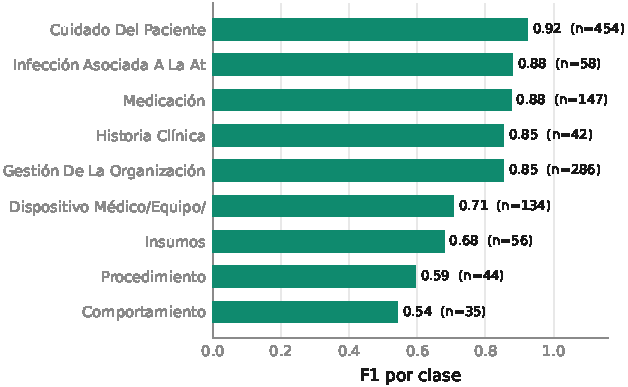
\includegraphics[width=\columnwidth]{figuras/fig4_ersp_clases.pdf}
\caption{Desempeño por naturaleza del evento sobre el corpus en español con
etiqueta de oro. El número de casos de prueba acompaña a cada clase: las de
menor F1 son también las de menor soporte.}
\label{fig:ersp}
\end{figure}

\subsection{Discusión}
El desglose completo se representa en la Figura~
ef{fig:ersp}. Las clases
con peor desempeño son \emph{Comportamiento} (F1 0.542),
\emph{Procedimiento} (0.595) e \emph{Insumos} (0.679), las tres con menos de 60
casos de prueba: el limitante es el número de ejemplos, no el método.

Estas cifras \textbf{no} son comparables con las de la
Tabla~\ref{tab:cascada}, y conviene ser explícito para evitar una lectura
errónea. El texto ERSP son descripciones breves ---unos 120 caracteres---
redactadas por alguien que \emph{ya identificó} el evento y lo está notificando;
la epicrisis son unos 17\,500 caracteres en los que el evento debe
\emph{localizarse} entre el resto de la historia. La tarea del ERSP es más
sencilla por construcción, y su mejor rendimiento no indica un modelo
superior sino un problema distinto.

Lo que sí demuestran es doble: que la taxonomía nacional es aprendible con
etiqueta humana experta, y que existe una vía de transferencia del sistema al
español que no depende de traducir el corpus en inglés.

\section{De la detección a la gestión: priorización y responsable}
\label{sec:gemses}

Detectar y clasificar un evento no lo gestiona. Un servicio de calidad que
recibiera varios miles de detecciones anuales sin criterio de ordenación
quedaría igual de inoperante que con el subregistro actual. El canal se
completa por tanto con dos etapas que traducen la salida del clasificador en
una decisión de gestión: \textbf{priorizar} y \textbf{asignar responsable}.

\subsection{Operacionalización de la matriz de priorización}
La priorización no emplea un criterio propio sino el instrumento normativo
vigente: la \emph{Matriz de Priorización de Impactos en Salud}, que la
Directiva N.º 7-OGCyH-ESSALUD-2020 cita en su artículo 5.13 como herramienta de
gestión. Esto sitúa el aporte del trabajo en el lugar correcto: no propone una
métrica de prioridad, sino que \emph{automatiza el cálculo} de una que la
institución ya reconoce.

Para cada tipo de evento $i$ se calculan cinco magnitudes:

\begin{align}
A_i &= \text{frecuencia observada} \\
B_i &= \frac{A_i}{\sum_j A_j} \times 9 \\
G_i &= 0{,}40\,c_i + 0{,}20\,d_i + 0{,}15\,e_i + 0{,}25\,f_i \\
H_i &= B_i \times G_i \qquad
I_i = \frac{H_i}{\sum_j H_j} \qquad
J_i = I_i \times 100
\end{align}

\noindent donde $c$ es la prolongación de estancia, $d$ las complicaciones
intrahospitalarias, $e$ los sobrecostos por no calidad y $f$ la insatisfacción
e imagen institucional, valoradas en la escala ordinal del instrumento
(muy alto 9, alto 6, medio 3, bajo 1, nulo 0). $B$ traslada la frecuencia
relativa a la escala de nueve puntos; $G$ pondera el impacto; $J$ expresa la
prioridad como porcentaje del impacto total.

Las tres primeras dimensiones son derivables de MIMIC-IV: la prolongación de
estancia se obtiene de las fechas de ingreso y alta, las complicaciones de los
propios eventos detectados y los sobrecostos como proxy de la estancia y los
procedimientos adicionales. La cuarta ---insatisfacción--- no tiene
correlato en el registro clínico y requiere valoración institucional, lo que
constituye una limitación declarada del despliegue automático.

\subsection{Bandas de prioridad y una degeneración corregida}
Las bandas se establecen sobre $J$ por percentiles: verde por debajo de $P_{25}$,
amarillo hasta $P_{75}$ y rojo por encima. Este criterio, correcto con
carteras amplias de eventos, \textbf{se degenera con pocos eventos distintos}:
los percentiles se comprimen y llegan a invertir la prioridad. En pruebas con
$n < 8$ se observó que una úlcera por presión de impacto $G = 6{,}3$ quedaba
clasificada en verde mientras un evento de $G = 2{,}3$ resultaba rojo.

La implementación incorpora una salvaguarda: por debajo de ocho eventos
distintos abandona los percentiles y aplica un corte absoluto sobre el impacto
($G \geq 6$ rojo, $G \geq 3$ amarillo). Verificado sobre el mismo caso, la
úlcera pasa a rojo y el evento menor a verde. El criterio empleado se registra
junto al resultado, de modo que toda priorización declara cómo se obtuvo.

\subsection{Asignación del responsable}
El último eslabón traduce la banda en un nivel de la pirámide de gestión, que
es lo que convierte un hallazgo en una acción con destinatario
(Tabla~\ref{tab:responsable}).

\begin{table}[htbp]
\caption{Asignación de responsable según banda de prioridad}
\label{tab:responsable}
\centering
\footnotesize
\begin{tabular}{@{}lp{0.62\columnwidth}@{}}
\toprule
\textbf{Banda} & \textbf{Nivel de gestión responsable} \\
\midrule
Verde & Nivel I: áreas operativas y servicios de salud \\
Amarillo & Nivel II: departamentos a cargo de los procesos transversales de las cadenas de valor \\
Rojo & Nivel III: varios departamentos, bajo liderazgo de la máxima autoridad del establecimiento \\
\bottomrule
\end{tabular}
\end{table}

La lógica es de escalamiento: un evento aislado de bajo impacto se resuelve
donde ocurre, mientras que uno de alta prioridad involucra procesos
transversales y exige conducción institucional. La asignación es determinista y
auditable ---no interviene ningún modelo---, lo que resulta deseable en un
componente que reparte responsabilidad.

\subsection{Clasificación según la jerarquía normativa}
En paralelo, cada detección se clasifica según el artículo 5 de la Directiva:
\emph{incidente} cuando no hubo daño, \emph{evento adverso} cuando lo hubo, y
\emph{evento centinela} ante muerte o daño permanente que exija tratamiento
permanente.

Dos precisiones sobre el alcance en MIMIC-IV. El \textbf{incidente queda fuera
de alcance}: por definición no causa daño y un resumen de alta no documenta
cuasi-fallas, que solo existen en un sistema de notificación voluntaria. El
\textbf{evento centinela sí es detectable} a partir del desenlace registrado
---mortalidad hospitalaria, destino al alta, traqueostomía o diálisis de
novo--- y es la categoría de mayor valor para un tablero de gestión, porque
concentra los casos que exigen investigación obligatoria.

\subsection{Estado de la integración}
Las tres etapas están implementadas y verificadas de forma independiente. El
presente informe reporta con detalle la primera (detección y clasificación) por
ser la que constituye el objeto del curso; la evaluación cuantitativa
\emph{de extremo a extremo} de la cadena completa ---incluyendo el acuerdo
entre la prioridad calculada y la que asignaría un comité de calidad---
permanece pendiente y se declara como tal.

\section{Limitaciones}
\begin{enumerate}
\item \textbf{Estándar de plata.} Las métricas sobre MIMIC miden acuerdo con
etiquetas derivadas de códigos CIE y no con juicio clínico; un falso positivo
puede ser la detección correcta de un evento no codificado.
\item \textbf{Reutilización del conjunto de prueba.} La misma partición se
evaluó a lo largo de las sucesivas iteraciones, lo que introduce un sesgo
optimista no cuantificado. El umbral de decisión no se ajustó.
\item \textbf{Alcance de la validación experta.} La muestra de revisión está
restringida a eventos de infección, de modo que $\kappa$ y el VPP corregido se
enuncian sobre ese subconjunto.
\item \textbf{Cobertura de datos estructurados.} Las tablas de cuidados
intensivos cubren el 19.7\,\% de las epicrisis, lo que limita cualquier regla
basada en signos vitales.
\item \textbf{Independencia del anotador.} El autor es a la vez desarrollador
del modelo y anotador de referencia. Se mitiga con interfaz ciega, orden
aleatorio, registro automático del tiempo por caso y estimación de la
fiabilidad contra un evaluador independiente.
\end{enumerate}

\section{Conclusiones}
El resultado con mayor valor de este trabajo es negativo y se dirige contra su
propia versión anterior: la conclusión de que un modelo léxico superaba a los
transformers clínicos \textbf{no resistió el control de las condiciones de
comparación}. Dos asimetrías no declaradas ---la ventana de contexto y la
ponderación de clases--- explicaban la ventaja atribuida al modelo simple. A
igualdad de ambas, el transformer ajustado no queda por debajo.

Lo que sí resiste es el efecto de la \textbf{ventana de contexto}: truncar el
texto a lo que el transformer alcanza a leer degrada al propio modelo léxico
con la misma arquitectura y los mismos datos. Dado que el modelo accede al
9.0\% de la epicrisis, la vía de mejora es una
arquitectura de secuencia larga \cite{cliniclong}, \cite{longformer} y no un
preentrenamiento clínico más específico.

En el plano metodológico, el aporte central es la \textbf{auditoría de validez
del etiquetado}: siete modos de fallo con efecto cuantificado, y el confusor
de época como caso ejemplar de aprendizaje por atajo ---un AUC de 0.973
sostenido en el reconocimiento de una plantilla documental--- que la corrección
redujo a 0.843 sobre una señal genuinamente clínica.

La \textbf{evaluación en cascada} muestra que reportar la clasificación
aislada sobreestima el rendimiento operativo en 34\,\%. La
\textbf{validación con un evaluador independiente} sitúa el valor puntual de
la concordancia en la banda sustancial, con la reserva del tamaño muestral. El
\textbf{corpus en español con etiqueta de oro} abre la transferencia a la
taxonomía nacional, y la \textbf{integración con la matriz de priorización}
(Sección~\ref{sec:gemses}) convierte la detección en una decisión de gestión
con responsable asignado, que es el destino aplicado del sistema.

\begin{thebibliography}{99}
\footnotesize

% --- corpus y acceso a datos
\bibitem{mimic4} A. E. W. Johnson, L. Bulgarelli, L. Shen, \emph{et al.},
``MIMIC-IV, a freely accessible electronic health record dataset,''
\emph{Scientific Data}, vol. 10, art. 1, 2023.
\bibitem{mimic3} A. E. W. Johnson, T. J. Pollard, L. Shen, \emph{et al.},
``MIMIC-III, a freely accessible critical care database,''
\emph{Scientific Data}, vol. 3, art. 160035, 2016.
\bibitem{physionet} A. L. Goldberger, L. A. N. Amaral, L. Glass,
\emph{et al.}, ``PhysioBank, PhysioToolkit, and PhysioNet,''
\emph{Circulation}, vol. 101, no. 23, pp. e215--e220, 2000.

% --- arquitectura y modelos de lenguaje
\bibitem{vaswani} A. Vaswani, N. Shazeer, N. Parmar, \emph{et al.},
``Attention is all you need,'' en \emph{Advances in Neural Information
Processing Systems (NeurIPS)}, 2017.
\bibitem{bert} J. Devlin, M.-W. Chang, K. Lee y K. Toutanova, ``BERT:
Pre-training of deep bidirectional transformers for language understanding,''
en \emph{Proc. NAACL-HLT}, 2019, pp. 4171--4186.
\bibitem{clinicalbert} E. Alsentzer, J. Murphy, W. Boag, \emph{et al.},
``Publicly available clinical BERT embeddings,'' en \emph{Proc. 2nd Clinical
Natural Language Processing Workshop}, NAACL, 2019, pp. 72--78.
\bibitem{biobert} J. Lee, W. Yoon, S. Kim, \emph{et al.}, ``BioBERT: a
pre-trained biomedical language representation model for biomedical text
mining,'' \emph{Bioinformatics}, vol. 36, no. 4, pp. 1234--1240, 2020.
\bibitem{pubmedbert} Y. Gu, R. Tinn, H. Cheng, \emph{et al.},
``Domain-specific language model pretraining for biomedical natural language
processing,'' \emph{ACM Trans. Computing for Healthcare}, vol. 3, no. 1,
pp. 1--23, 2021.
\bibitem{huang} K. Huang, J. Altosaar y R. Ranganath, ``ClinicalBERT:
Modeling clinical notes and predicting hospital readmission,''
\emph{arXiv:1904.05342}, 2019.
\bibitem{beto} J. Cañete, G. Chaperon, R. Fuentes, \emph{et al.},
``Spanish pre-trained BERT model and evaluation data,'' en \emph{PML4DC at
ICLR}, 2020.

% --- ventana de contexto y documentos largos
\bibitem{longformer} I. Beltagy, M. E. Peters y A. Cohan, ``Longformer: The
long-document transformer,'' \emph{arXiv:2004.05150}, 2020.
\bibitem{bigbird} M. Zaheer, G. Guruganesh, A. Dubey, \emph{et al.}, ``Big
Bird: Transformers for longer sequences,'' en \emph{NeurIPS}, 2020.
\bibitem{cliniclong} Y. Li, R. M. Wehbe, F. S. Ahmad, H. Wang y Y. Luo,
``Clinical-Longformer and Clinical-BigBird: Transformers for long clinical
sequences,'' \emph{arXiv:2201.11838}, 2022.

% --- métodos léxicos y herramientas
\bibitem{sklearn} F. Pedregosa, G. Varoquaux, A. Gramfort, \emph{et al.},
``Scikit-learn: Machine learning in Python,'' \emph{J. Machine Learning
Research}, vol. 12, pp. 2825--2830, 2011.
\bibitem{fasttext} A. Joulin, E. Grave, P. Bojanowski y T. Mikolov, ``Bag of
tricks for efficient text classification,'' en \emph{Proc. EACL}, 2017,
pp. 427--431.
\bibitem{hf} T. Wolf, L. Debut, V. Sanh, \emph{et al.}, ``Transformers:
State-of-the-art natural language processing,'' en \emph{Proc. EMNLP: System
Demonstrations}, 2020, pp. 38--45.

% --- supervisión débil y negación
\bibitem{snorkel} A. Ratner, S. H. Bach, H. Ehrenberg, \emph{et al.},
``Snorkel: Rapid training data creation with weak supervision,'' \emph{Proc.
VLDB Endowment}, vol. 11, no. 3, pp. 269--282, 2017.
\bibitem{negex} W. W. Chapman, W. Bridewell, P. Hanbury, G. F. Cooper y
B. G. Buchanan, ``A simple algorithm for identifying negated findings and
diseases in discharge summaries,'' \emph{J. Biomedical Informatics}, vol. 34,
no. 5, pp. 301--310, 2001.

% --- fiabilidad entre observadores
\bibitem{cohen} J. Cohen, ``A coefficient of agreement for nominal scales,''
\emph{Educational and Psychological Measurement}, vol. 20, no. 1, pp. 37--46,
1960.
\bibitem{landis} J. R. Landis y G. G. Koch, ``The measurement of observer
agreement for categorical data,'' \emph{Biometrics}, vol. 33, no. 1,
pp. 159--174, 1977.
\bibitem{byrt} T. Byrt, J. Bishop y J. B. Carlin, ``Bias, prevalence and
kappa,'' \emph{J. Clinical Epidemiology}, vol. 46, no. 5, pp. 423--429, 1993.
\bibitem{feinstein} A. R. Feinstein y D. V. Cicchetti, ``High agreement but
low kappa: I. The problems of two paradoxes,'' \emph{J. Clinical
Epidemiology}, vol. 43, no. 6, pp. 543--549, 1990.
\bibitem{sim} J. Sim y C. C. Wright, ``The kappa statistic in reliability
studies: use, interpretation, and sample size requirements,'' \emph{Physical
Therapy}, vol. 85, no. 3, pp. 257--268, 2005.
\bibitem{efron} B. Efron y R. J. Tibshirani, \emph{An Introduction to the
Bootstrap}. Nueva York: Chapman \& Hall, 1993.

% --- validez, sesgos y aprendizaje por atajo
\bibitem{geirhos} R. Geirhos, J.-H. Jacobsen, C. Michaelis, \emph{et al.},
``Shortcut learning in deep neural networks,'' \emph{Nature Machine
Intelligence}, vol. 2, pp. 665--673, 2020.
\bibitem{zech} J. R. Zech, M. A. Badgeley, M. Liu, \emph{et al.}, ``Variable
generalization performance of a deep learning model to detect pneumonia in
chest radiographs: A cross-sectional study,'' \emph{PLoS Medicine}, vol. 15,
no. 11, e1002683, 2018.

% --- seguridad del paciente y detección de eventos adversos
\bibitem{brennan} T. A. Brennan, L. L. Leape, N. M. Laird, \emph{et al.},
``Incidence of adverse events and negligence in hospitalized patients,''
\emph{New England J. Medicine}, vol. 324, no. 6, pp. 370--376, 1991.
\bibitem{kohn} L. T. Kohn, J. M. Corrigan y M. S. Donaldson (eds.),
\emph{To Err Is Human: Building a Safer Health System}. Washington, DC:
National Academies Press, 2000.
\bibitem{classen} D. C. Classen, R. Resar, F. Griffin, \emph{et al.},
``Global Trigger Tool shows that adverse events in hospitals may be ten times
greater than previously measured,'' \emph{Health Affairs}, vol. 30, no. 4,
pp. 581--589, 2011.
\bibitem{murff} H. J. Murff, F. FitzHenry, M. E. Matheny, \emph{et al.},
``Automated identification of postoperative complications within an electronic
medical record using natural language processing,'' \emph{JAMA}, vol. 306,
no. 8, pp. 848--855, 2011.
\bibitem{who} World Health Organization, \emph{Global Patient Safety Action
Plan 2021--2030: Towards eliminating avoidable harm in health care}. Ginebra:
WHO, 2021.

% --- normativa institucional
\bibitem{directiva02} EsSalud, \emph{Directiva de Eventos Adversos},
GG-ESSALUD-2021, Anexo 02: taxonomía de eventos adversos; Anexo 03: escala de
severidad.
\bibitem{directiva7} EsSalud, \emph{Directiva N.º 7-OGCyH-ESSALUD-2020}:
gestión del reporte de eventos adversos y seguridad del paciente.
\bibitem{cifras} EsSalud, \emph{EsSalud en Cifras: Informativo Mensual},
edición definitiva de diciembre de 2025, publicada el 26 de marzo de 2026.
Estadística Institucional. [En línea]. Disponible en:
\url{https://www.gob.pe/institucion/essalud/informes-publicaciones/6505357-essalud-en-cifras-informativo-mensual-2025}
\end{thebibliography}

\end{document}
